\section{wrapup}

\section*{Angewendeter iterativ-inkrementeller Softwareentwicklungsprozess in SWEN1/PM3}
\begin{itemize}
  \item Der Softwareentwicklungsprozess wurde so angepasst (engl. tailoring), dass die wesentlichen Artefakte in einem Softwareprojekt im Kontext eingeführt werden können.
  \item Die Software wird in Iterationen entwickelt (2 Wochen Rhythmus).
  \item Jede Iteration hat ein Ziel und wird nach Abschluss reviewed.
  \item Es gibt drei Meilensteine, die im Projektverlauf ein besonderes Ereignis darstellen bzw. den Abschluss einer Phase: Projektskizze (M1), Lösungsarchitektur (M2) und Beta-Release (M3)
  \item In jeder Iteration werden Anforderungen, Analyse \& Design, Implementation und Testing gemacht (Software entsteht in Inkrementen).
  \item Der angewendete Softwareentwicklungsprozess und das Projektmanagement eines iterativ-inkrementellen Projektes wird in PM3 noch detaillierter erklärt.
\end{itemize}

\section*{Wesentliche Resultate bzw. Artefakte}
\begin{itemize}
  \item Anforderungsanalyse
  \item Funktionale Anforderungen mit Use Cases
  \item Qualitätsanforderungen und Randbedingungen
  \item Domänenmodell
  \item Design
  \item Softwarearchitektur
  \item Use Case Realisierung (statische und dynamische Modelle)
  \item Implementation
  \item Quellcode (inkl. Javadoc)
  \item Testing
  \item Unit-Tests\\
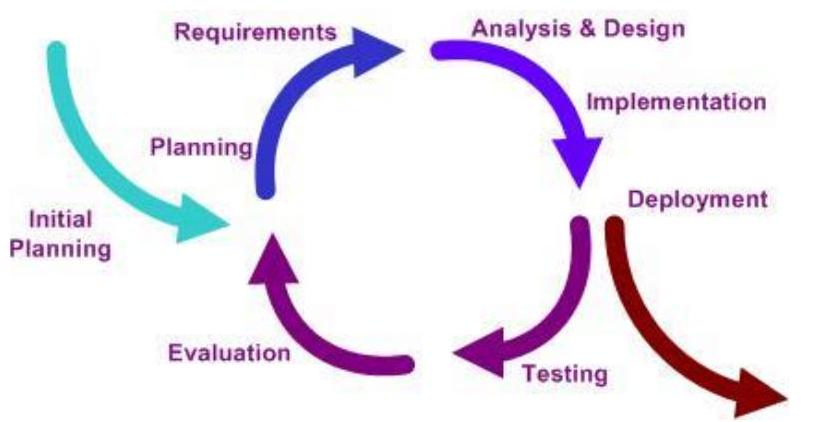
\includegraphics[max width=\textwidth, center]{2025_01_02_6eafa38dd4ae10c9a392g-09}
  \item Integrations- und Systemtests
\end{itemize}

\section*{Modellierung und Modelle mit der UML}

\includegraphics[max width=\textwidth, center]{2025_01_02_6eafa38dd4ae10c9a392g-10}\\
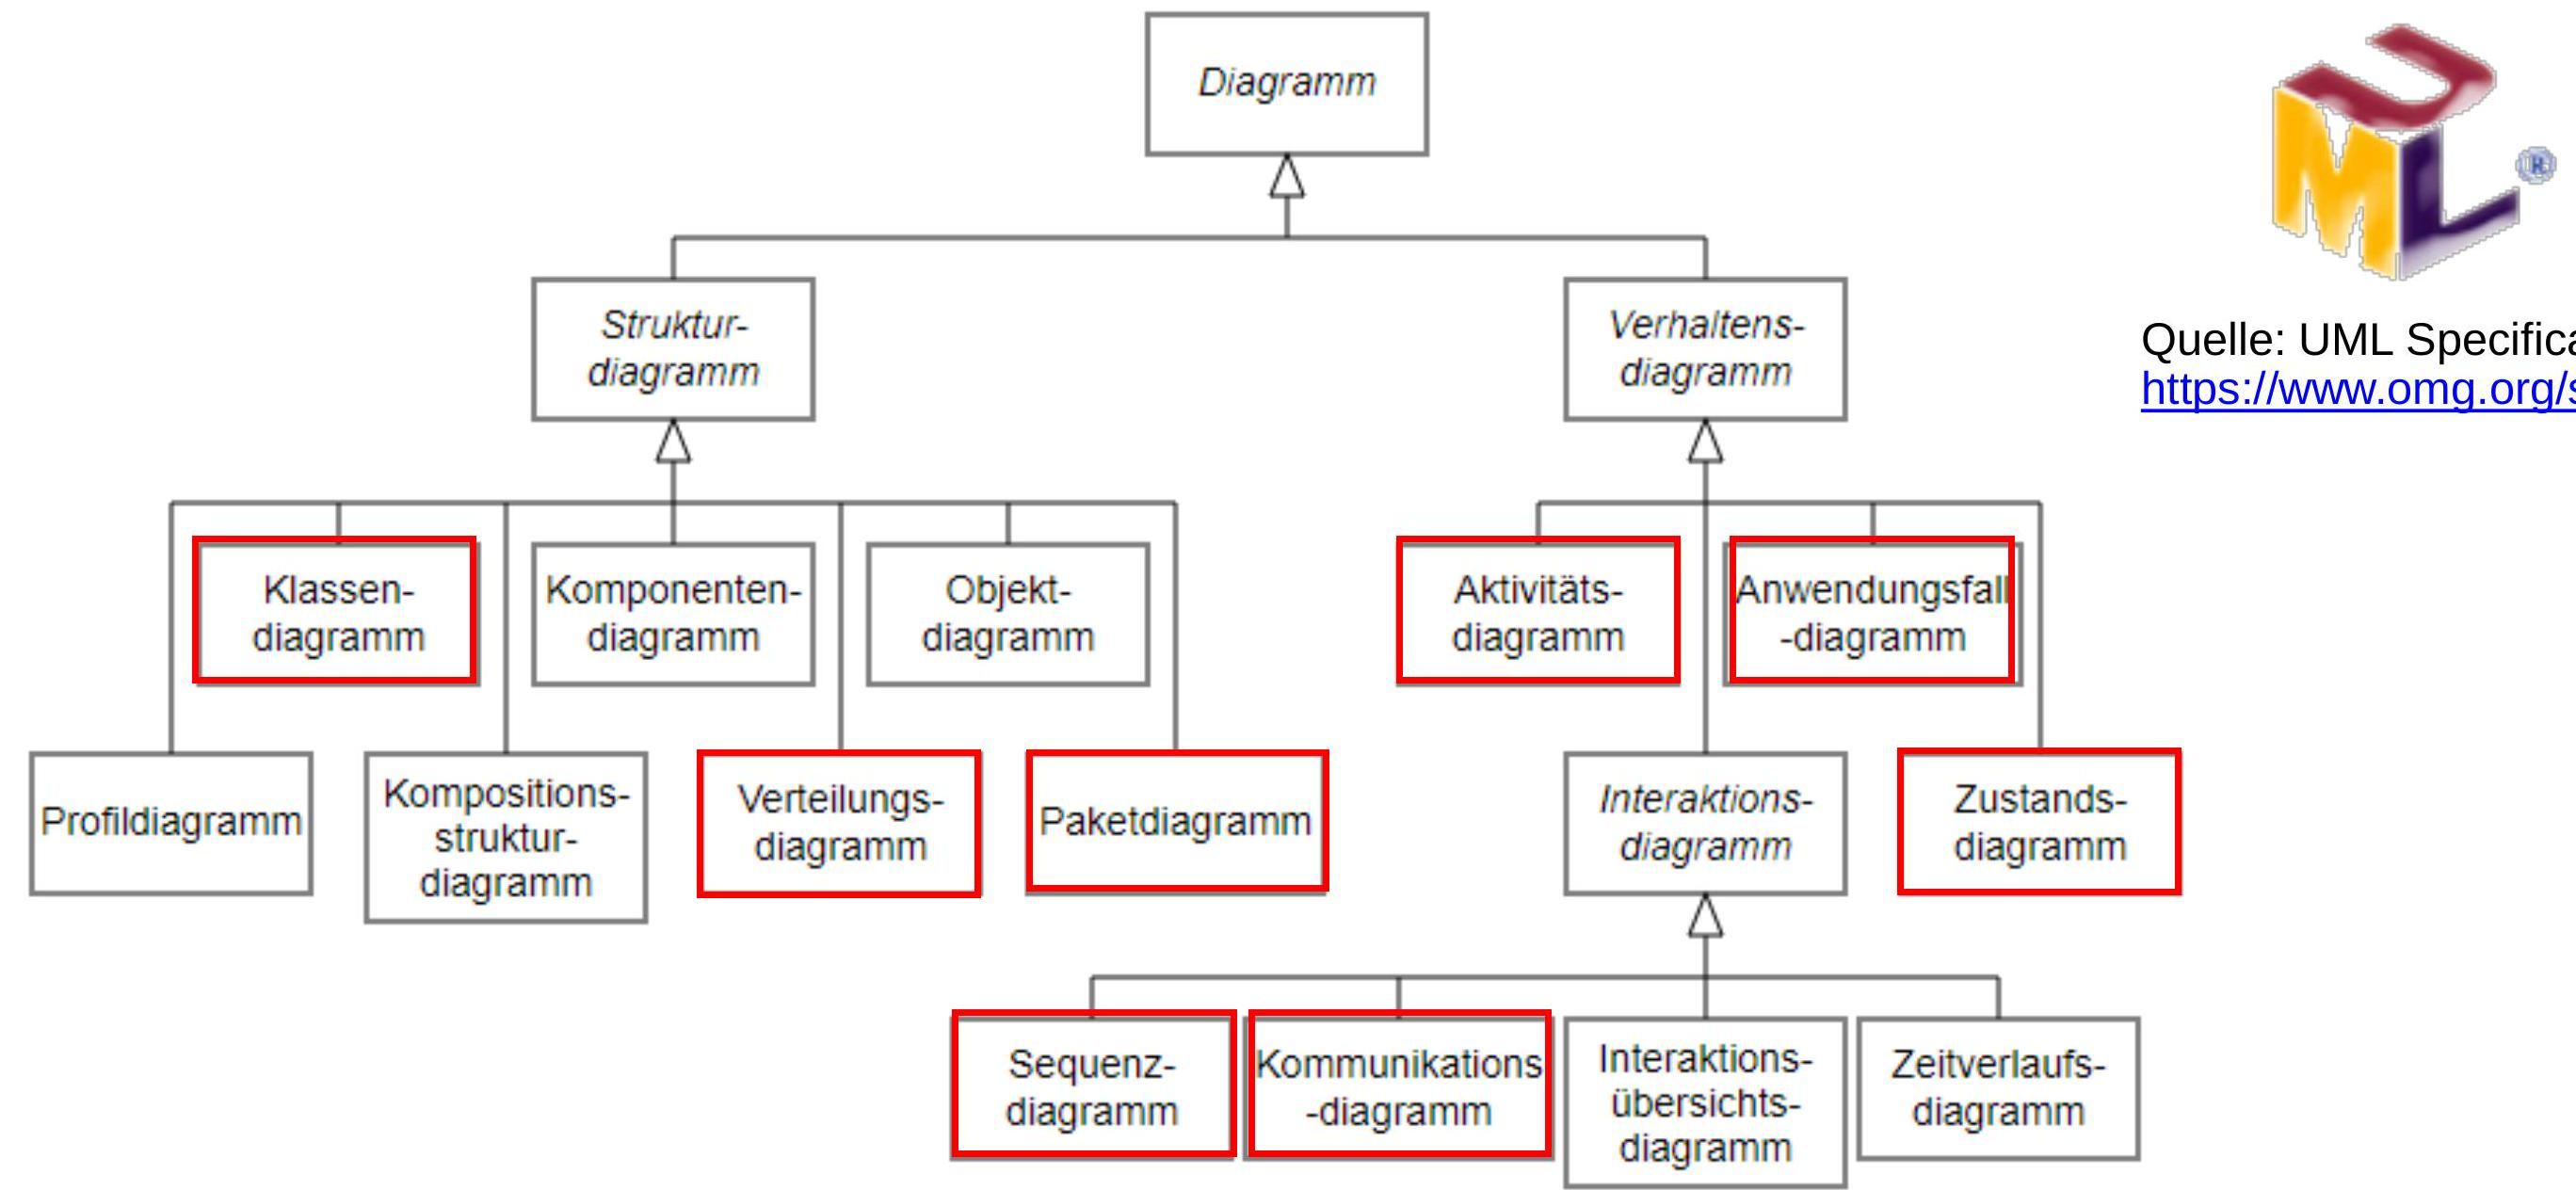
\includegraphics[max width=\textwidth, center]{2025_01_02_6eafa38dd4ae10c9a392g-10(1)}

Quelle: UML Specification, \href{https://www.omg.org/spec/UML/}{https://www.omg.org/spec/UML/}\\
$\square$ für die Modellierung in SWEN1 relevant

\section*{Gebrauch der UML (nach Martin Fowler)}
\section*{- UML as a Sketch}
\begin{itemize}
  \item Informelle und unvollständige Diagramme (z.T. von Hand gezeichnet), um schwierige Teile des Problems oder der Lösung zu verstehen und zu kommunizieren
  \item Die agile Community bevorzugt diese Anwendungsart von UML
  \item UML as a Blueprint
  \item Relativ detaillierte Analyse und Design-Diagramme für Code-Generierung oder um existierenden Code besser zu verstehen
  \item Klassische UML-Tools für ein Forward- und Reverse-Engineering (Roundtrip)
  \item UML as a Programming Language
  \item Komplete, ausführbare Spezifikation eines Software-Systems in UML
  \item MDA-Tools zur Modellierung und Generierung
\end{itemize}

\section*{Überblick Anforderungen \& Analyse}
\begin{itemize}
  \item User Research (Personas und Szenarien, Contextual Inquiry)
  \item Sketching und Protoyping
  \item Ableiten und Modellieren von Use Cases (dt. Anwendungsfälle)
  \item Detaillierung der Use Case (UML-Use-Case-Diagramm, Use-CaseSpezifikationen, UI-Sketching
  \item Qualitätsanforderungen und Randbedingungen erheben und festhalten.
  \item Modellierung der Fachlichkeit und Begriffe des Anwenders in einem Domänenmodell (konzeptuelles UML-Klassendiagramm)
  \item Bei der objektorientierten Analyse (OOA) liegt die Betonung darauf, die Objekte - oder Konzepte in dem Problembereich zu finden und zu beschreiben!
\end{itemize}

\section*{Überblick Design}
\begin{itemize}
  \item Design und Modellierung einer für die Problemstellung geeigneten Softwarearchitektur (UML-Paketdiagramm, UML-Verteilungsdiagramm)
  \item Use-Case-Realisierung und Klassendesign mit Verantwortlichkeiten (UML-Klassendiagramm, UML-Sequenzdiagramm, UMLKommunikationsdiagramm, UML-Zustandsdiagramm, UML-\\
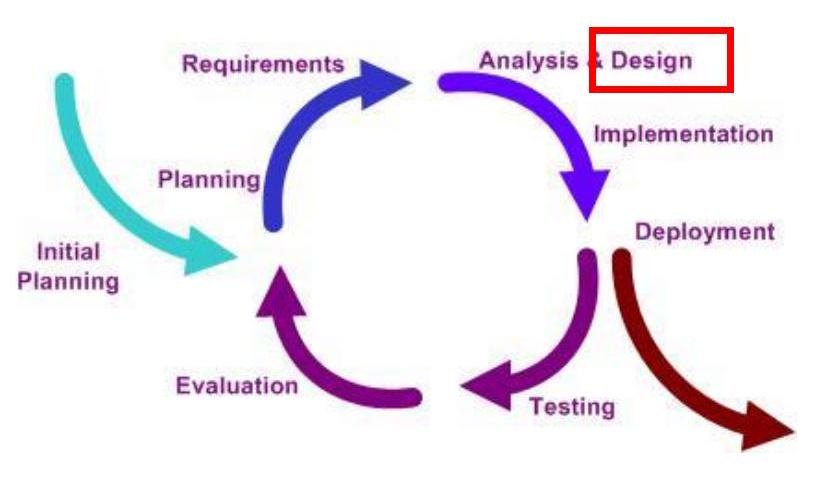
\includegraphics[max width=\textwidth]{2025_01_02_6eafa38dd4ae10c9a392g-13} Aktivitätsdiagramm)
  \item Entwurf mit bewährten Design Patterns
  \item Beim objektorientierten Design (OOD) liegt die Betonung darauf, geeignete Softwareobjekte und ihr Zusammenwirken (engl. collaboration) zu definieren, um die Anforderungen zu erfüllen!
\end{itemize}

\section*{Überblick Implementation}
\begin{itemize}
  \item Umsetzung des Designs in Code der entsprechenden (objektorientierten) Programmiersprache
  \item Verwendung von geeigneten Algorithmen und Datenstrukturen zur Implementierung des Designs
  \item Code Smells sofort bei deren Aufdeckung verbessern (Refactoring)\\
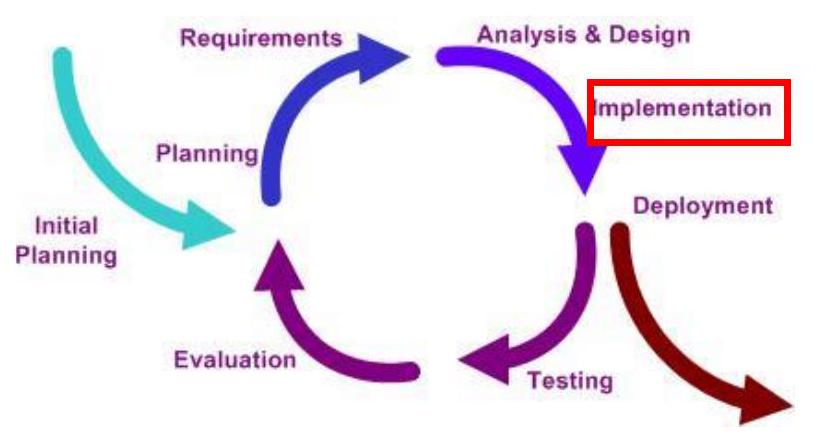
\includegraphics[max width=\textwidth, center]{2025_01_02_6eafa38dd4ae10c9a392g-14}
  \item Laufende Dokumentation des Quellcodes (nach Clean CodePrinzipien)
\end{itemize}

\section*{Überblick Testing}
\begin{itemize}
  \item Laufendes Design und Implementierung von Unit-Tests
  \item Planung, Design und Durchführung von weiteren Tests auf den Teststufen Integration und System je nach Problemstellung
  \item Dokumentation des Testkonzepts und der Tests\\
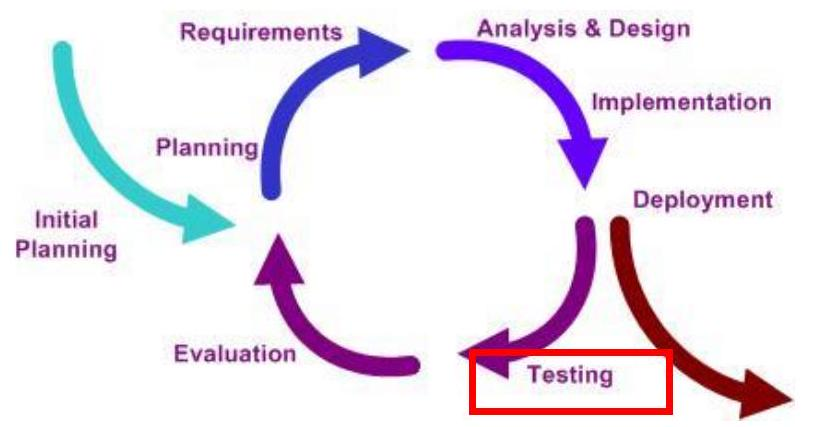
\includegraphics[max width=\textwidth, center]{2025_01_02_6eafa38dd4ae10c9a392g-15}
\end{itemize}